\documentclass[12pt]{article}

\usepackage[utf8]{inputenc}
\usepackage[T2A]{fontenc}
\usepackage[english,russian]{babel}
\usepackage{amssymb}
\usepackage{graphicx}
\graphicspath{ {images/} }

\textwidth=431pt
\textheight=600pt
\hoffset=-15pt
\voffset=-15pt

\usepackage{graphicx}
\usepackage{amsmath}
\makeatletter
\renewcommand{\@oddhead}{%
\vbox{%
\hbox to \textwidth{\strut \textit{CV, Assignment 1, Usvyatsov Mikhail} \hfill }
%\hbox to\textwidth{Лист\hfill Страница~\arabic{page}~из 2}
\hrule
\vspace{12pt}
}}
\renewcommand{\@oddfoot}{}
\makeatother

\begin{document}
	
	\bigskip
	\textbf{Algorithm}
	
	First step is to understand what is happaning from the samples.
	
	For each sample image we:\\

	\begin{enumerate}
		\item split the image into RGB channels;
		
		\item subtract G and B components from the doubled R component to measure the prevalence of red component over green and blue ones.
		
		$$lightness_{RED}:=2R-G-B$$
		
		Experiments show, that due to constant parameters of the light we can distinct every of three classes from the brightness of red channel.
		
		\item Calculate the average value of all pixels in $lightness_{RED}$.
		\item Compare average lightens with learn thresholds.
	\end{enumerate}
	
	After the train step we do the following:
	
	For each image in test set:
	
	\begin{enumerate}
		\item Load test image;
		\item Split the test image into channels;
		\item Find $lightness_{RED}$ for the image;
		\item Calculate the average value of all pixels in $lightness_{RED}$;
		\item Compare average lightens with learned thresholds.
	\end{enumerate}
	
	\newpage
	
	\textbf{Illustration}
	
	Here are a few results of image spliting:\\
	
	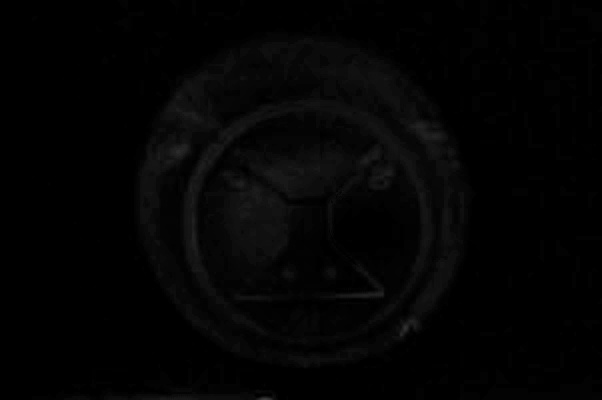
\includegraphics[width=1\textwidth]{result}\\
	
	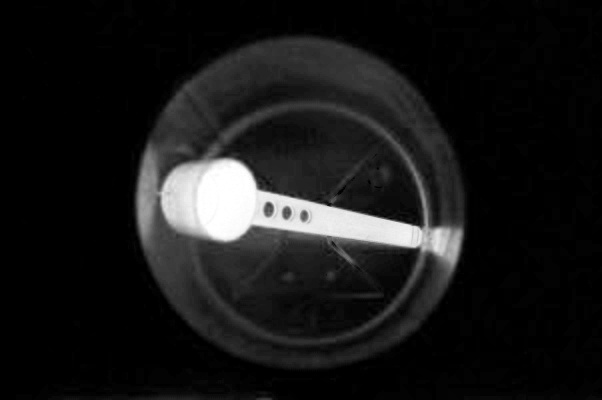
\includegraphics[width=1\textwidth]{result1}\\
	
	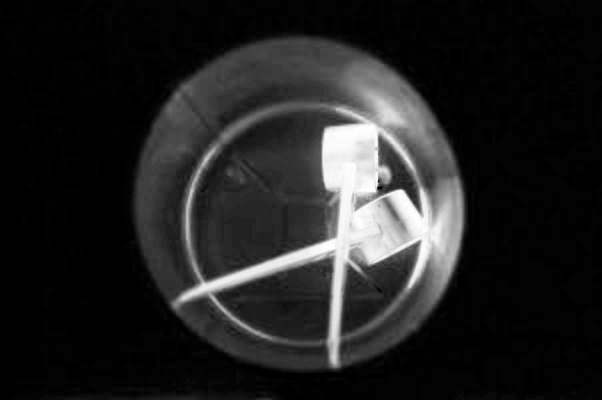
\includegraphics[width=1\textwidth]{result2}\\
	
	From upside down: $lightness_{RED}$.
	\medskip
	
	\textbf{Performance measure}
	According to confusion matrix:
	
	\begin{tabular}{|c||c|c|c|}
		\hline
		\ & predicted 1 & predicted 0 & Total \\
		\hline
		real class 1 & True Positive (TP) & False Negative (FN) & P\\
		\hline
		real class 0 & False Positive (FP) & True Negative (TN) & N \\
		\hline
		Total & $P'$ & $N'$ & $P+N$\\
		\hline 
	\end{tabular}
	\medskip
	
	The formulas for precision, recall and accuracy:
	\newcounter{ecounter}
	\begin{list}{\arabic{ecounter})~}{\usecounter{ecounter}}
		\item $precision = \dfrac{TP}{TP+FP}$
		\item $recall = \dfrac{TP}{P}$
		\item $accuracy = \frac{TP+TN}{P+N}$
	\end{list}
	\newpage
	
	The results of the program:

	For every class precision = recall = accuracy = 100%
	
\end{document}